\documentclass[a4paper, 10pt]{article}
\linespread{1.33}
% ┌─────────────────────┐
% │     preamble.tex    │
% └─────────────────────┘

% ══════════ [1] Basic document settings ══════════
\usepackage{fullpage}
\usepackage{geometry}
\geometry{
    top = 2cm,
    bottom = 4.5cm,
    left = 2.5cm,
    right = 2.5cm
}
\usepackage{lastpage}

\usepackage{xcolor}
\usepackage{graphicx}
\usepackage{tikz}
\usepackage{pgfplots}

\usepackage{enumerate}
\usepackage{sectsty}
\subsectionfont{\color{blue}}
\usepackage{enumitem}
\usepackage{array}
\newcolumntype{P}[1]{>{\centering\arraybackslash}p{#1}}

\usepackage{fourier-orns}
\usetikzlibrary{decorations.text}
\pgfplotsset{compat = newest}
\newcommand{\seprule}{
    \vspace*{1.5em}
    \vspace{-8pt}\hrulefill
    \raisebox{-2.1pt}{\quad\decofourleft\decotwo\decofourright\quad}\hrulefill
    \vspace*{1.5em}
}

\usepackage{hyperref}
\hypersetup{
  colorlinks=true,
  linkcolor=blue,
  linkbordercolor={0 0 1},
  urlcolor=blue
}

\usepackage{fancyhdr}
\usepackage[]{mdframed}

\renewcommand{\thesubsection}{\S{} \arabic{section}.\arabic{subsection}}

% ══════════ [2] Math packages ══════════
\usepackage{amsmath}
\usepackage{amsthm}
\usepackage{amsfonts}
\usepackage{amssymb}
\usepackage{amscd}
\usepackage{mathrsfs}
\usepackage{cancel}

% ══════════ [3] Miscellaneous & Fonts ══════════
\setlength{\parindent}{0.0in}
\setlength{\parskip}{0.05in}
\renewcommand{\footrulewidth}{0.4pt}

\usepackage{mathpazo}
\usepackage{domitian}
\usepackage[T1]{fontenc}
\let\oldstylenums\oldstyle
\setmonofont[Scale = 0.8]{DejaVu Sans Mono}

% ══════════ [4] amsthm setup ══════════

\newtheorem{theorem}{Theorem}[section]
\newtheorem{corollary}[theorem]{Corollary}
\newtheorem{lemma}[theorem]{Lemma}

\theoremstyle{definition}
\newtheorem{definition}[theorem]{Definition}

\theoremstyle{remark}
\newtheorem*{remark}{Remark}

\theoremstyle{definition}
\newtheorem{obs}[theorem]{Observation}

\theoremstyle{definition}
\newtheorem{exercise}[theorem]{Exercise}
\newmdtheoremenv[innertopmargin = 8pt,
                 innerbottommargin = 10pt]{exer}[theorem]{Exercise}

\theoremstyle{definition}
\newtheorem{example}[theorem]{Example}
% ┌─────────────────────┐
% │   usercommand.tex   │
% └─────────────────────┘

% ══════════ [1] short-hand notations ══════════
\newcommand{\mbf}{\mathbf}
\newcommand{\mrm}{\mathrm}
\newcommand{\mca}{\mathcal}
\newcommand{\msc}{\mathsc}
\newcommand{\mbb}{\mathbb}
\newcommand{\msf}{\mathsf}

\newcommand{\tbf}{\textbf}
\newcommand{\tit}{\textit}

\newcommand{\eps}{\epsilon}
\newcommand{\kB}{k_{\mathrm{B}}}
\def\dbar{{\mathchar'26\mkern-12mu d}}
\newcommand{\contradiction}{\ensuremath{{\Rightarrow\mspace{-2mu}\Leftarrow}}}
\newcommand{\im}{\mathrm{im}\,}
\renewcommand{\d}{\mathrm{d}}

\renewcommand\qedsymbol{$\blacksquare$}

\newcommand\lecturenumber{05}
\newcommand\lecturedate{Nov 8, 2024}

\pagestyle{fancyplain}
\headheight 40pt
\lhead{Lecture \lecturenumber\\CNBC Deep Learning Subgroup}
\rhead{Riemannian Geometry for Deep Learning \\\lecturedate}
\cfoot{Fall 2024, SNU}
\rfoot{\small\thepage}
\headsep 1.5em

\begin{document}
\setcounter{section}{3}
\section{Manifolds: Definitions}

\setcounter{subsection}{2}
\subsection{Manifolds}

\setcounter{theorem}{16}
\begin{definition}
    $M$ is a $m$-dimensional \tbf{differential manifold} if
    \begin{itemize}
        \item[(i)] $M$ is a \tit{topological space}.
        \item[(ii)] $M$ is provided with a family of pairs $\{ (U_{i}, \varphi_{i}) \}$ such that
        \item[(iii)] $\{ U_{i} \}$ is a family of open sets which covers $M$ ($\displaystyle{\cup_{i} U_{i} = M}$) and $\varphi_{i}$ is a \tit{homeomorphism} from $U_{i}$ onto an open subset $U_{i}' \subseteq \mbb{R}^{m}$.
        \item[(iv)] For $U_{i} \cap U_{j} \neq \varnothing$, the \tbf{transition function} $\psi_{ij} = \varphi_{i} \circ \varphi_{j}^{-1}$ from $\varphi_{j}(U_{i} \cap U_{j})$ to $\varphi_{i}(U_{i} \cap U_{j})$ is $C^{\infty}$.
    \end{itemize}
    \begin{figure}[htbp!]
        \centering
        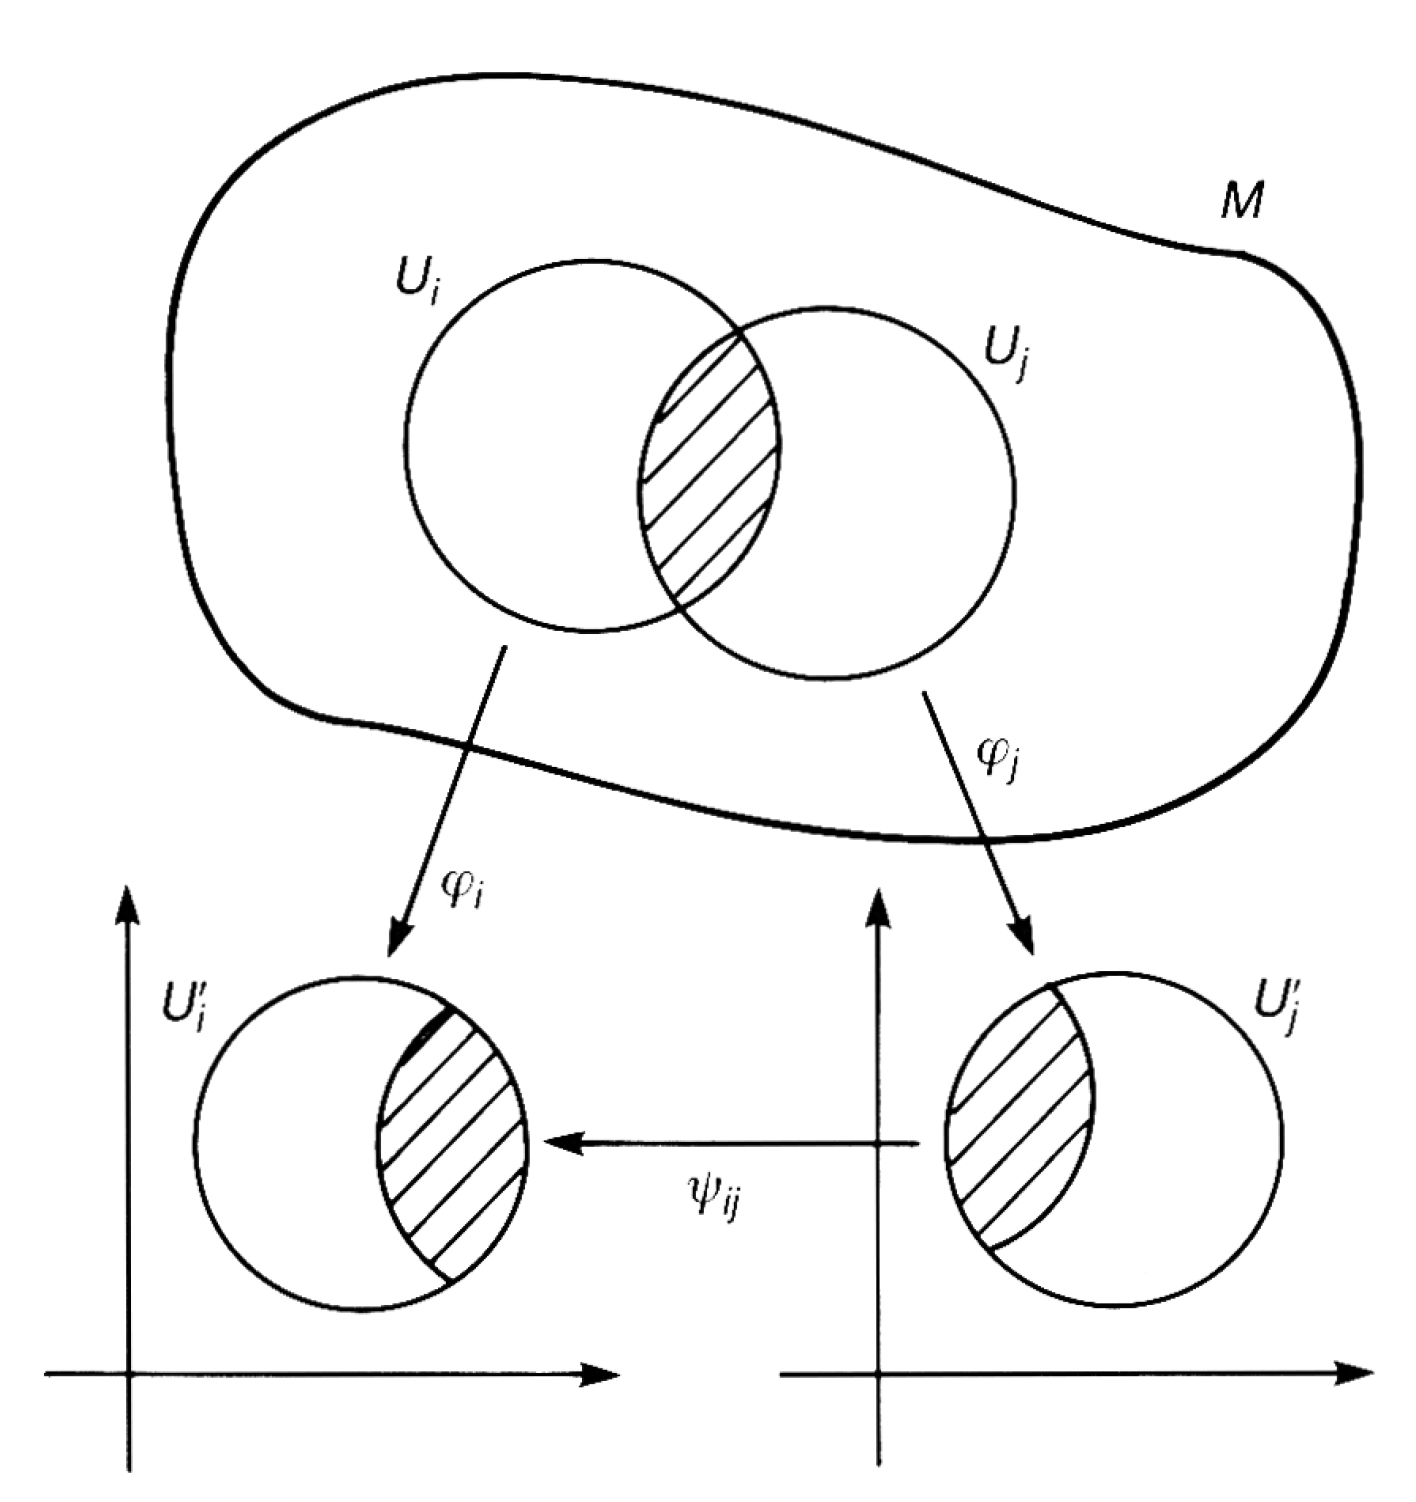
\includegraphics[width=0.4\linewidth]{../images/lecture05/5_01.png}
    \end{figure}
\end{definition}

\begin{remark}
    \hphantom{.}
    \begin{itemize}
        \item[(1)] We call $U_{i}$ and $\varphi_{i}$ \tbf{coordinate neighborhood} and \tbf{coordinate function}, respectively. The tuple $(U_{i}, \varphi_{i})$ is called a \tbf{chart}. Collection of charts, $\{ (U_{i}, \varphi_{i}) \}$ is called an \tbf{atlas}. The coordinate function is
        \[ \varphi_{i}(p) = (x^{1}(p),\, x^{2}(p),\, \cdots,\, x^{m}(p))  \]
        \item[(2)] From (ii) and (iii), $M$ is \tbf{LOCALLY} Euclidean(in each coordinate neighborhood $U_{i}$, $M$ looks like an open set of $\mbb{R}^{m}$ - of course $M \neq \mbb{R}^{m}$ globally).
        \item[(3)] From (iv), transition from one coordinate system to another should be smooth(or $C^{\infty}$). Consider a point $p \in U_{i} \cap U_{j}$. Then corresponding coordinate functions $\varphi_{i}$ and $\varphi_{j}$ assign $x^{\mu}$ and $y^{\mu}$ respectively. The transition $x^{\mu} = x^{\mu}(y^{\alpha})$ should be $C^{\infty}$.
    \end{itemize}
\end{remark}

\begin{remark}
    If the union of two atlases $\{ (U_{i}, \varphi_{i}) \}$ and $\{ (V_{j}, \psi_{j}) \}$ is again an atlas, these two atlases are said to be \tbf{compatible}. Such compatibility gives rise to \tit{equivalence relations}. Equivalence classes are called \tbf{differentiable structures} on $M$.
\end{remark}
\newpage

% ===== ===== ===== ===== ===== ===== ===== ===== ===== ===== ===== =====

\begin{example}
    Examples of manifolds.
    \begin{itemize}
        \item[(a)] $\mbb{R}^{n}$ is a trivial example: single chart covers whole $\mbb{R}^{n}$, with $\varphi$ as an identity map.
        \item[(b)] $S^{1}$, a circle $x^{2} + y^{2} = 1$ in the $xy$-plane is another example.
        
        \begin{figure}[htbp]
            \centering
            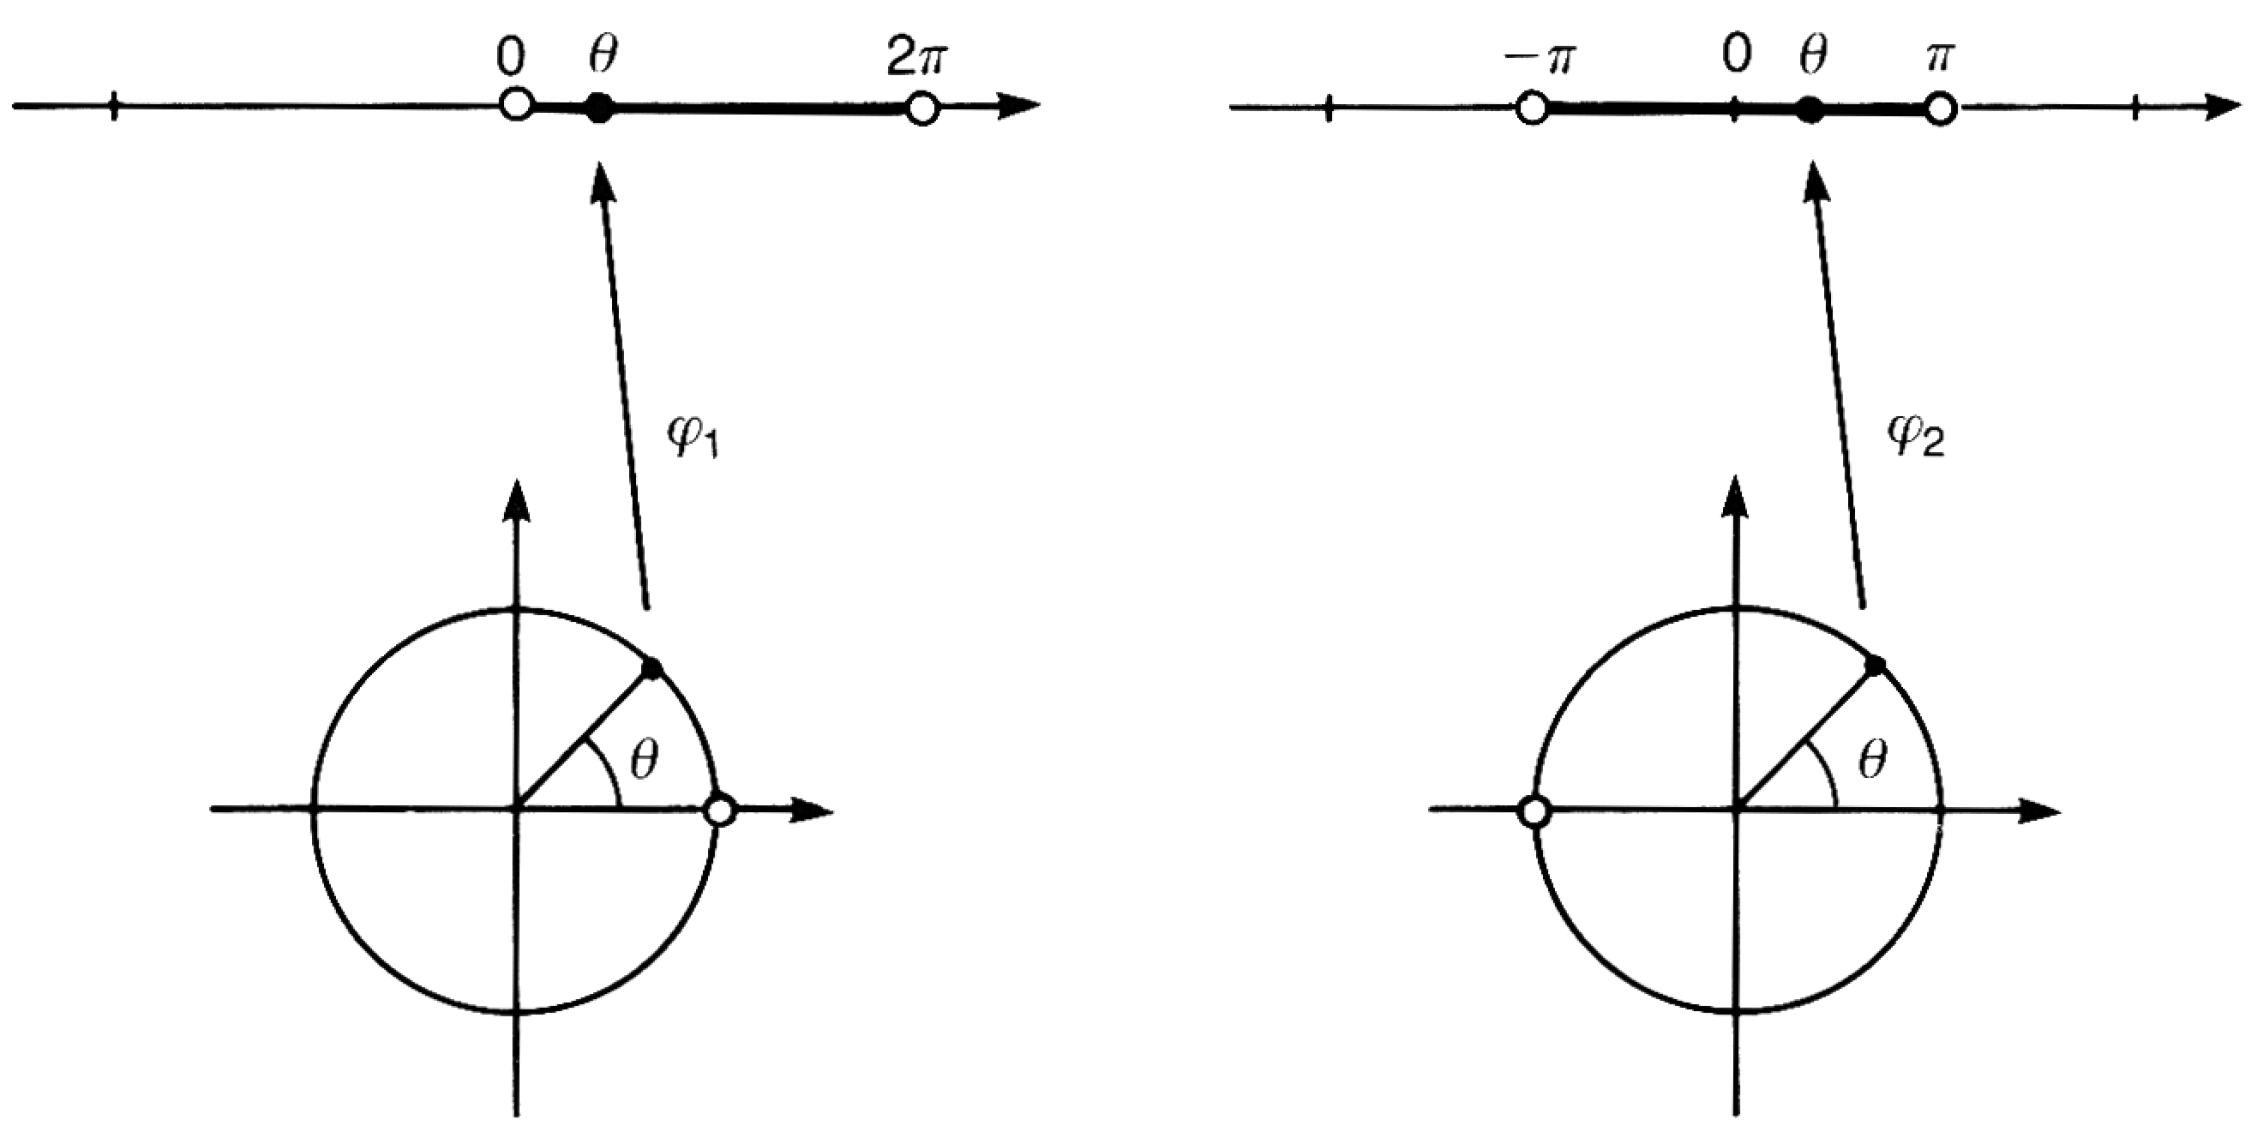
\includegraphics[width=0.8\linewidth]{../images/lecture05/5_02.png}
        \end{figure}
        
        For two open sets $U_{1} = (0, 2\pi)$ and $U_{2} = (-\pi,\pi)$,
        \begin{align*}
            \varphi_{1}^{-1} \,:\, U_{1} \rightarrow S^{1}-\{(1,0)\} &\quad\text{s.t.}\quad \theta \mapsto (\cos\theta,\,\sin\theta) \\
            \varphi_{2}^{-1} \,:\, U_{2} \rightarrow S^{1}-\{(-1,0)\} &\quad\text{s.t.}\quad \theta \mapsto (\cos\theta,\,\sin\theta)
        \end{align*}
        One can show that:
        \begin{itemize}
            \item[-] $\varphi_{1}^{-1}$ and $\varphi_{2}^{-1}$ are invertible.
            \item[-] $\varphi_{1},\,\varphi_{1}^{-1},\,\varphi_{2},\,\varphi_{2}^{-1}$ are continuous\footnote{From these two conditions, $\varphi_{1}$ and $\varphi_{2}$ become \tit{homeomorphisms}}.
            \item[-] $\psi_{12} = \varphi_{1} \circ \varphi_{2}^{-1}$ and $\psi_{21} = \varphi_{2} \circ \varphi_{1}^{-1}$ are smooth.
        \end{itemize}
        \item[(c)] $S^{n}$ realized in $\mbb{R}^{n+1}$: $\displaystyle{\sum_{i=0}^{n}(x^{i})^{2} = 1}$. Define coordinate neighborhoods
        \begin{align*}
            U_{i+} &= \{ (x^{0},\, x^{1},\, \cdots,\, x^{n}) \,|\, x^{i} > 0\} \\
            U_{i-} &= \{ (x^{0},\, x^{1},\, \cdots,\, x^{n}) \,|\, x^{i} < 0\}
        \end{align*}
        and coordinate maps by
        \begin{align*}
            \varphi_{i+} \,:\, U_{i+} \rightarrow \mbb{R}^{n}, &\quad \varphi_{i+}(x^{0},\, \cdots,\, x^{n}) = (x^{0},\,\cdots,\,x^{i-1},\,x^{i+1},\,\cdots,\,x^{n}) \\
            \varphi_{i-} \,:\, U_{i-} \rightarrow \mbb{R}^{n}, &\quad \varphi_{i-}(x^{0},\, \cdots,\, x^{n}) = (x^{0},\,\cdots,\,x^{i-1},\,x^{i+1},\,\cdots,\,x^{n})
        \end{align*}
        These are projections of the hemispheres $U_{i\pm}$ to the plane $x^{i} = 0$. For example, we can consider $U_{x\pm},\,U_{y\pm}$ and $U_{z\pm}$ for $S^{2}$. Then, one transition function of this atlas becomes
        \begin{align*}
            \psi_{y-x+} &:= \varphi_{y-} \circ \varphi_{x+}^{-1} \\
            \psi_{y-x+}(y,z) &= (\sqrt{1-y^{2}-z^{2}},z)
        \end{align*}
        which is $\mca{C}^{\infty}$ on $U_{x+} \cap U_{y-}$.
        \item[(d)] \tbf{Stereographic projections}. Construct the atlas by
        \begin{itemize}
            \item[-] $S^{2}-\{\text{South Pole}\}$ with stereographic projection from South Pole
            \item[-] $S^{2}-\{\text{North Pole}\}$ with stereographic projection from North Pole
        \end{itemize}
        Then, transition function is smooth (show this as an exercise).
    \end{itemize}
\end{example}

\seprule

\begin{example}
    The \tbf{real projective space} $\mbb{R}P^{n}$ is the set of lines through the origin in $\mbb{R}^{n+1}$.
    \begin{itemize}
        \item[-] If $x = (x^{0},\, \cdots,\, x^{n}) \neq 0$, $x$ defines a line through the origin.
        \item[-] $y \in \mbb{R}^{n+1}$ defines the same line as $x$ if $\exists\,a\neq 0\;\text{s.t.}\;y=ax$.
        \item[-] Hence, we can define an \tit{equivalence relation} by
        \[ x\sim y \;\Longleftrightarrow\; \exists\,a\in\mbb{R}-\{0\}\;\text{s.t.}\;y=ax \]
        \item[-] From the equivalence relation, a quotient space with equivalence classes can be defined.
        \[ \mbb{R}P^{n} := (\mbb{R}^{n+1}-\{0\})/\sim \]
        \item[-] Since $\mbb{R}P^{n} \subset \mbb{R}^{n+1}$, it has $(n+1)$-coordinates $x^{0},\,\cdots,\,x^{n}$, which is not good(since $\mbb{R}P^{n}$ is an $n$-dimensional manifold). These are \tbf{homogeneous} coordinates.
    \end{itemize}
    Let $U_{i}$ be set of lines with $x^{i} \neq 0$. Then, \tbf{inhomogeneous} coordinates on $U_{i}$ is defined by
    \[ \xi_{(i)}^{j} = \frac{x^{j}}{x^{i}},\; \xi_{(i)} = (\xi_{(i)}^{0},\,\xi_{(i)}^{1},\,\cdots,\,\xi_{(i)}^{i-1},\,\xi_{(i)}^{(i+1)},\,\cdots,\,\xi_{(i)}^{n}) \]
    This coordinate system is independent of the choice of the representative.
    \[ \frac{x^{j}}{x^{i}} = \frac{y^{j}}{y^{i}} \;\text{where}\;y = ax \]
    The coordinate map corresponding to the chart becomes
    \[ \varphi_{i} \,:\, (x^{0},\,\cdots,\,x^{n}) \mapsto (\frac{x^{0}}{x^{i}},\,\cdots,\,\frac{x^{i-1}}{x^{i}},\,\frac{x^{i+1}}{x^{i}},\,\cdots,\,\frac{x^{n}}{x^{i}}) \]
    For $x \in U_{i} \cap U_{j}$ (with inhomogeneous coordinates $\xi_{(i)}^{k} = \frac{x^{k}}{x^{i}}$ and $\xi_{(j)}^{k} = \frac{x^{k}}{x^{j}}$), transition function
    \[ \psi_{ij} \,:\, \xi_{(j)}^{k} \rightarrow \mapsto \xi_{(i)}^{k} = \frac{x^{j}}{x^{i}}\xi_{(j)}^{k} \]
    is smooth.
\end{example}

\begin{remark}
    The real projective space can be generalized into $k$-dimensional planes in $\mbb{R}^{n}$. Such planes also form \tbf{Grassmann manifold} $G_{k,n}(\mbb{R})$.
\end{remark}
\newpage

% ===== ===== ===== ===== ===== ===== ===== ===== ===== ===== ===== =====

\begin{definition}[Product manifold]
    Let $M$ and $N$ be $m$- and $n$-dimensional manifold with atlases $\{(U_{i},\varphi_{i})\}$ and $\{(V_{j},\psi_{j})\}$, respectively. The \tbf{product manifold} $M\times N$ is a $(m+n)$-dimensional manifold whose atlas is $\{(U_{i}\times V_{j}),\,(\varphi_{i},\psi_{j})\}$.
\end{definition}

\begin{example}
    Consider the \tbf{torus} $T^{2} = S^{1} \times S^{1}$.
    
    \begin{figure}[htbp]
        \centering
        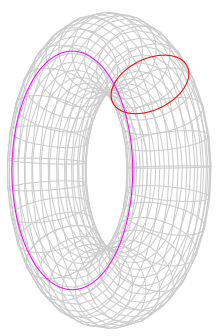
\includegraphics[width=0.3\linewidth]{../images/lecture05/5_03.png}
    \end{figure}

    \begin{itemize}
        \item[-] The torus can be described by two coordinates $(\theta_{1},\theta_{2})$.
        \item[-] Since $S^{1}$ is embedded in $\mbb{R}^{2}$, we can imagine $T^{2}$ embedded in $\mbb{R}^{4}$. This is the torus as a \tit{flat} manifold.
        \item[-] However, we often imagine $T^{2}$ as the surface of a doughnut in $\mbb{R}^{3}$, in which case, however, we inevitably have to introduce bending of the surface.
        \item[-] This is the \tbf{extrinsic} feature brought about by the embedding.
        \item[-] In the \tbf{intrinsic} point of view, we forget about the embedding. More on this later.
    \end{itemize}
\end{example}

In summary,
\begin{center}
    Manifolds are LOCALLY homeomorphic to Euclidean spaces $\mbb{R}^{n}$,\\
    enabling differentiation and integration on them.
\end{center}
\newpage

% ===== ===== ===== ===== ===== ===== ===== ===== ===== ===== ===== =====

\subsection{Differentiable Maps}

\begin{definition}[Differentiable maps]
    Let $f \,:\, M \rightarrow N$ be a map from an $m$-dimensional manifold $M$ to an $n$-dimensional manifold $N$.
    
    \begin{figure}[htbp]
        \centering
        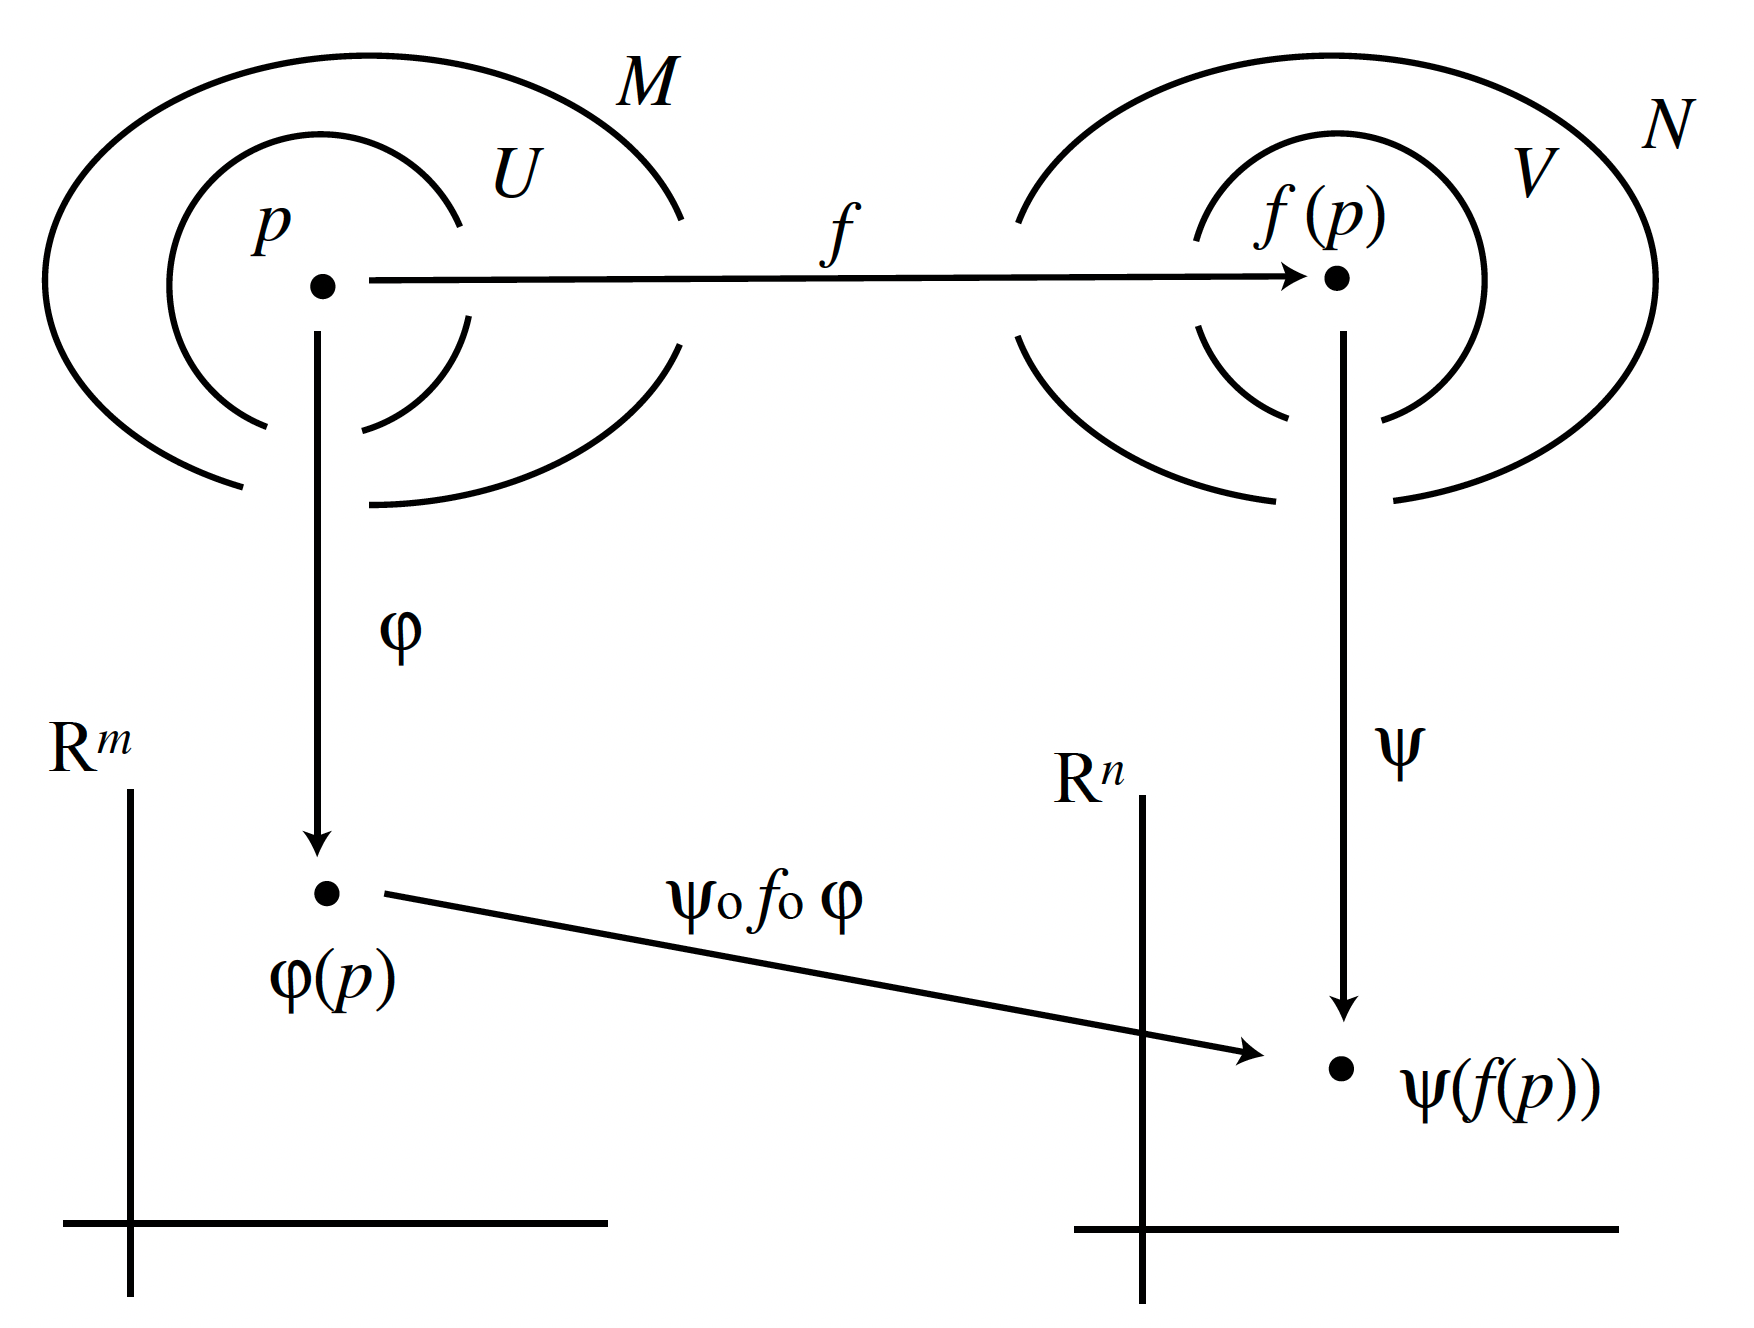
\includegraphics[width=0.4\linewidth]{../images/lecture05/5_04.png}
    \end{figure}
    
    Take a chart $(U,\varphi)$ on $M$ and $(V,\psi)$ on $N$. Then $f$ has the coordinate representation
    \[ \psi \circ f \circ \varphi^{-1} \,:\, \mbb{R}^{m} \rightarrow \mbb{R}^{n} \]
    If we write $\varphi(p) = (x^{\mu})$ and $\psi(f(p)) = (y^{\alpha})$, $\psi\circ f\circ\varphi^{-1}(x) = y$. We often \tit{abuse} the notation as
    \[ y = f(x),\; y^{\alpha} = f^{\alpha}(x^{\mu}) \]
    If $\psi\circ f\circ\varphi^{-1}$ is smooth with respect to each $x^{\mu}$, $f$ is said to be \tbf{differentiable}(or \tbf{smooth}) at $p$.
\end{definition}

\begin{remark}
    The differentiability of $f$ is independent of coordinate system. Consider a overlapping charts $(U_{1},\varphi_{1})$ and $(U_{2},\varphi_{2})$ with $p \in U_{1} \cap U_{2}$ and
    \[ \varphi_{1}(p) = (x_{1}^{\mu}),\; \varphi_{2}(p) = (x_{2}^{\nu}) \]
    where $f$ is differentiable with first chart. Then
    \[ \psi\circ f\circ \varphi_{2}^{-1} = (\underbrace{\psi\circ f\circ\varphi_{1}^{-1}}_{\mca{C}^{\infty}})\circ(\underbrace{\varphi_{1}\circ\varphi_{2}^{-1}}_{=\psi_{12},\;\mca{C}^{\infty}}) \]
    $f$ is also differentiable in second chart.
\end{remark}

\begin{definition}[Diffeomorphism]
    Let $f \,:\, M \rightarrow N$ be a homeomorphism and $\psi$ and $\varphi$ be coordinate functions as previously defined. If $\psi\circ f\circ\varphi^{-1}$ is invertible and both $y = \psi\circ f\circ \varphi^{-1}(x)$ and $x = \varphi\circ f\circ\psi^{-1}(y)$ are $\mca{C}^{\infty}$, $f$ is called a \tbf{diffeomorphism} and $M$ is said to be \tbf{diffeomorphic} to $N$ and vice versa, denoted by $M\equiv N$.
\end{definition}

\begin{remark}
    $M\equiv N$ implies $\dim M = \dim N$.
\end{remark}
\begin{remark}
    \tit{Homeomorphisms} classify spaces according to whether it is possible to deform one space into another \tit{continuously}. \tit{Diffeomorphisms} classify spaces into equivalence classes according to whether it is possible to deform one space into another \tit{smoothly}.
\end{remark}
\newpage

% ===== ===== ===== ===== ===== ===== ===== ===== ===== ===== ===== =====

\begin{definition}
    The set of diffeomorphisms $f \,:\, M \rightarrow M$ is a group denoted by $\mrm{Diff}(M)$.
\end{definition}

\begin{remark}
    Active and passive transformation point of view
    \begin{itemize}
        \item Take a point $p$ in a chart $(U, \varphi)$ such that $\varphi(p) = x^{\mu}(p)$. Under $f \in \mrm{Diff}(M)$, $p$ is mapped into $f(p)$ and $\varphi(f(p)) = y^{\mu}(f(p))$. Clearly $y$ is a differentiable function of $x$(\tbf{active} transformation).
        \item If $(U,\varphi)$ and $(V,\psi)$ are overlapping charts with $x^{\mu}=\varphi(p)$ and $y^{\mu} = \psi(p)$ ($p\in U\cap V$), the map $x \mapsto y$ is differentiable by the assumed smoothness of the manifold(\tbf{passive} transformation).
    \end{itemize}
\end{remark}

Before we finish, let me define two important entities for later.
\begin{definition}[Curves]
    An \tbf{open curve} in an $m$-dimensional manifold $M$ is a map $c\,:\,(a,b) \rightarrow M$ such that
    \begin{itemize}
        \item[-] $c$ does not intersect with itself.
        \item[-] For simplicity, we assume 0 is included in $(a,b)$.
        \item[-] $a$ and $b$ can be $-\infty$ and $\infty$, respectively.
    \end{itemize}
\end{definition}

\begin{definition}[Functions on the manifold]
    A \tbf{function} $f$ on $M$ is a smooth map $f \,:\, M \rightarrow \mbb{R}$. The set of smooth functions on $M$ is denoted by $\mca{F}(M)$.
\end{definition}

\end{document}
